\chapter{Revision History}
\label{Chp:RevHistory}
%--------------------------------------------------------------

Changes in 2.0.0:
\begin{itemize}
\item (Issue xx) [PENDING] Introduction of {\sf GrB\_Scalar}.
\item (Issue 70,67) [PENDING] changes to {\sf GrB\_wait(obj)}. {\sf GrB\_wait(void)} is removed from the specification breaking backward compatibility.
\item (Issue 74) [PENDING] assign integer values to all return codes.
\item (Issue 73) [PENDING] allow {\sf GrB\_NULL} for dup operator in matrix and vector {\sf build} methods.  Return error if duplicate locations encountered.
\item (Issue 34) [PENDING] Added new select operation with index unary operator. Added new variants of apply that take an index unary operator (matrix and vector variants).
\item (Issue 68) [PENDING] Added serialize and deserialize methods for matrices \scott{and vectors?}.
\item (Issue 51) [PENDING] Adding import and export methods for matrices
\item (Issue 69) Made names/symbols containing underscores searchable in PDF.
\item Typographical error in version macros was corrected.  They are all caps: {\sf GRB\_VERSION} and {\sf GRB\_SUBVERSION}.
\item Typographical change to eWiseAdd Description to be consistent in order of set intersections.
\item Typographical errors in eWiseAdd: cut-and-paste errors from eWiseMult/set intersection fixed to read eWiseAdd/set union.
\item Typographical error ({\sf NEQ} $\rightarrow$ {\sf NE}) in Description of Table~\ref{Tab:PredefinedTrueSemirings}.
\end{itemize}

%--------------------------------------------------------------

Changes in 1.3.0 (25 September 2019):
\begin{itemize}
\item (Issue 50) Changed definition of completion and added {\sf GrB\_wait()} that takes an opaque GraphBLAS object as an argument.
\item (Issue 39) Added {\sf GrB\_kronecker} operation.
\item (Issue 40) Added variants of the {\sf GrB\_apply} operation that take a binary function and a scalar.
\item (Issue 59) Changed specification about how reductions to scalar ({\sf GrB\_reduce}) are to be performed (to minimize dependence on monoid identity).
\item (Issue 24) Added methods to resize matrices and vectors ({\sf GrB\_Matrix\_resize} and {\sf GrB\_Vector\_resize}).
\item (Issue 47) Added methods to remove single elements from matrices and vectors ({\sf GrB\_Matrix\_removeElement} and {\sf GrB\_Vector\_removeElement}).
\item (Issue 41) Added {\sf GrB\_STRUCTURE} descriptor flag for masks (consider only the structure of the mask and not the values).
\item (Issue 64) Deprecated {\sf GrB\_SCMP} in favor of new {\sf GrB\_COMP} for descriptor values.
\item (Issue 46) Added predefined descriptors covering all possible combinations of field, value pairs.
\item Added unary operators: absolute value ({\sf GrB\_ABS\_$T$}) and bitwise complement of integers ({\sf GrB\_BNOT\_$I$}). 
\item (Issues 42,62) Added binary operators: Added boolean exclusive-nor ({\sf GrB\_LXNOR}) and bitwise logical operators on integers ({\sf GrB\_BOR\_$I$}, {\sf GrB\_BAND\_$I$}, {\sf GrB\_BXOR\_$I$}, {\sf GrB\_BXNOR\_$I$}).
\item (Issue 11) Added a set of predefined monoids and semirings.
\item (Issue 57) Updated all examples in the appendix to take advantage of new capabilities and predefined objects.
\item (Issue 43) Added parent-BFS example.
\item (Issue 1) Fixed bug in the non-batch betweenness centrality algorithm in 
Appendix~\ref{App:BCnobatch} where source nodes were incorrectly assigned path counts.
\item (Issue 3) Added compile-time preprocessor defines and runtime method for querying the GraphBLAS API version being used.
\item (Issue 10) Clarified {\sf GrB\_init()} and {\sf GrB\_finalize()} errors.
\item (Issue 16) Clarified behavior of boolean and integer division. {\color{red} Note that {\sf GrB\_MINV} for integer and boolean types was removed from this version of the spec.}
\item (Issue 19) Clarified aliasing in user-defined operators.
\item (Issue 20) Clarified language about behavior of {\sf GrB\_free()} with predefined objects (implementation defined)
\item (Issue 55) Clarified that multiplication does not have to distribute over addition in a GraphBLAS semiring.
\item (Issue 45) Removed unnecessary language about annihilators.
\item (Issue 61) Removed unnecessary language about implied zeros.
\item (Issue 60) Added disclaimer against overspecification.
\item Fixed miscellaneous typographical errors (such as $\otimes.\oplus$).
\end{itemize}

%--------------------------------------------------------------

Changes in 1.2.0:
\begin{itemize}
\item Removed "provisional" clause.
\end{itemize}

%--------------------------------------------------------------

Changes in 1.1.0:
\begin{itemize}
\item Removed unnecessary {\sf const} from {\sf nindices}, {\sf nrows}, and {\sf ncols} parameters of both {\sf extract} and {\sf assign} operations.
\item Signature of {\sf GrB\_UnaryOp\_new} changed: order of input parameters changed.
\item Signature of {\sf GrB\_BinaryOp\_new} changed: order of input parameters changed.
\item Signature of {\sf GrB\_Monoid\_new} changed: removal of domain argument which is now inferred from the domains of the binary operator provided.
\item Signature of {\sf GrB\_Vector\_extractTuples} and {\sf GrB\_Matrix\_extractTuples} to add an in/out argument, {\sf n}, which indicates the size of the output arrays provided (in terms of number of elements, not number of bytes).  Added new execution error, {\sf GrB\_INSUFFICIENT\_SPACE} which is returned when the capacities of the output arrays are insufficient to hold all of the tuples.
\item Changed {\sf GrB\_Column\_assign} to {\sf GrB\_Col\_assign} for consistency in non-polymorphic interface.
\item Added replace flag (z) notation to Table~\ref{Tab:GraphBLASOps}.
\item Updated the ``Mathematical Description" of the assign operation in Table~\ref{Tab:GraphBLASOps}.
\item Added triangle counting example.
\item Added subsection headers for accumulate and mask/replace discussions in the Description sections of GraphBLAS operations when the respective text was the ``standard" text (i.e., identical in a majority of the operations).
\item Fixed typographical errors.
\end{itemize}  

%--------------------------------------------------------------

Changes in 1.0.2:
\begin{itemize}
\item Expanded the definitions of {\sf Vector\_build} and {\sf Matrix\_build} to conceptually use intermediate matrices and avoid casting issues in certain implementations.
\item Fixed the bug in the {\sf GrB\_assign} definition. Elements of the output object are no longer being erased outside the assigned area.
\item Changes non-polymorphic interface:
    \begin{itemize}
    \item Renamed {\sf GrB\_Row\_extract} to {\sf GrB\_Col\_extract}.
    \item Renamed {\sf GrB\_Vector\_reduce\_BinaryOp} to {\sf GrB\_Matrix\_reduce\_BinaryOp}.
    \item Renamed {\sf GrB\_Vector\_reduce\_Monoid} to {\sf GrB\_Matrix\_reduce\_Monoid}.
    \end{itemize}
\item Fixed the bugs with respect to isolated vertices in the Maximal Independent Set example.
\item Fixed numerous typographical errors.
\end{itemize}

%--------------------------------------------------------------
%--------------------------------------------------------------

\chapter{Non-Opaque Data Format Definitions}
\label{Chp:GrB_Format}

\section{{\sf GrB\_Format}: Specify the format for input/output of a GraphBLAS matrix.}
\label{Sec:GrB_Format}

The type {\sf GrB\_Format} specifies the format of a non-opaque data type from
which data is to be imported from or exported into.  Here we define the
data formats that can be specified with {\sf GrB\_Format}.

\subsection{{\sf GrB\_CSR\_FORMAT}}

The {\sf GrB\_CSR\_FORMAT} format indicates that a matrix will be imported or
exported using the compressed sparse
row (CSR) format.  {\sf indptr} will be a pointer to an array of size nrows+1
and the i'th index will contain the starting index of the i'th row in the {\sf values}
and {\sf indices} arrays.  The elements of each row are not required to be sorted
by column index.
{\sf indices} will be a pointer to an array of size number of
stored elements, where each element contains the corresponding element's column index.
{\sf values} will be a pointer to an array of size number of
stored elements, where each element contains the corresponding value.\\

\begin{figure}[h]
    \hrule
    \begin{center}
        ~\\
        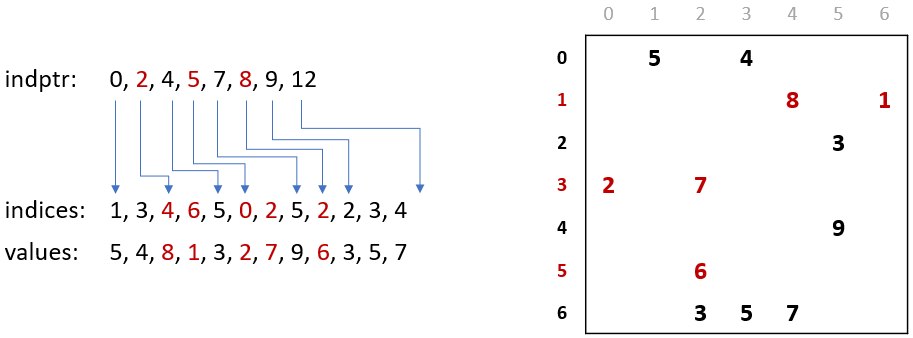
\includegraphics[width=4.5in]{GrB_CSR_FORMAT.png}
    \end{center}
    \caption{Data layout for CSR format.}
    \label{Fig:formats}
    \hrule
\end{figure}

\subsection{{\sf GrB\_CSC\_FORMAT}}

The {\sf GrB\_CSC\_FORMAT} format
indicates that a matrix will be imported or exported using the compressed sparse
column (CSC) format.  {\sf indptr} will be a pointer to an array of size ncols+1
and the i'th index will contain the starting index of the i'th column in the {\sf values}
and {\sf indices} arrays.  The elements of each column are not required to be
sorted by row index.
{\sf indices} will be a pointer to an array of size number of
stored elements, where each element contains the corresponding element's row index.
{\sf values} will be a pointer to an array of size number of
stored elements, where each element contains the corresponding element's value.\\

\begin{figure}[h]
    \hrule
    \begin{center}
        ~\\
        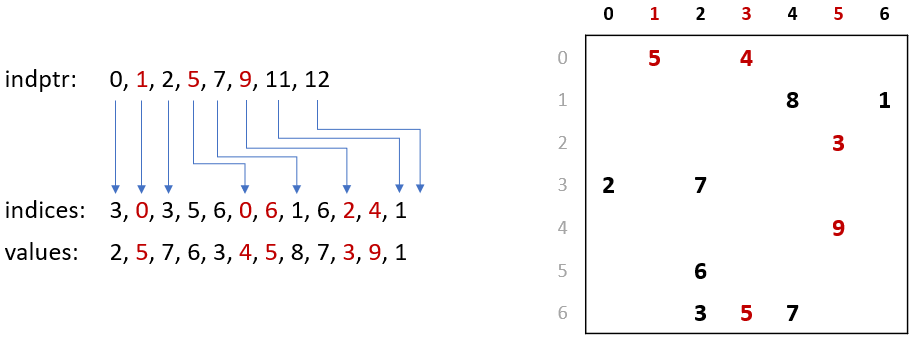
\includegraphics[width=4.5in]{GrB_CSC_FORMAT.png}
    \end{center}
    \vspace{-1em}
    \caption{Data layout for CSC format.}
    \hrule
\end{figure}

\subsection{{\sf GrB\_COO\_FORMAT}}

The {\sf GrB\_COO\_FORMAT} format
indicates that a matrix will be imported or exported using the coordinate list
(COO) format.  {\sf indptr} will be a pointer to an array of size number of stored elements,
where each element contains the corresponding element's column index.
{\sf indices} will be a pointer to an array of size number of stored elements, where each
element contains the corresponding element's row index.
{\sf values} will be a pointer to an array of size number of
stored elements, where each element contains the corresponding value. Elements
are not required to be sorted in any order.\\

\begin{figure}[h]
    \hrule
    \begin{center}
        ~\\
        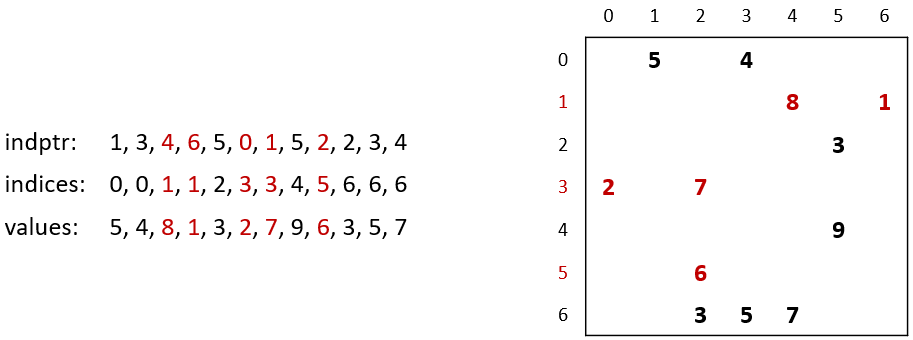
\includegraphics[width=4.5in]{GrB_COO_FORMAT.png}
    \end{center}
    \vspace{-1em}
    \caption{Data layout for COO format.}
    \hrule
\end{figure}

\subsection{{\sf GrB\_DENSE\_ROW\_FORMAT}}

The {\sf GrB\_DENSE\_ROW\_FORMAT} format indicates that a matrix will be imported
or exported using the dense row-major format.  {\sf indptr} and {\sf indices} are unused,
and may be set to NULL, while {\sf values} will point to an array of size number of columns
times number of rows, where element i,j is located at index i*ncols + j.\\

\begin{figure}[h]
    \hrule
    \begin{center}
        ~\\
        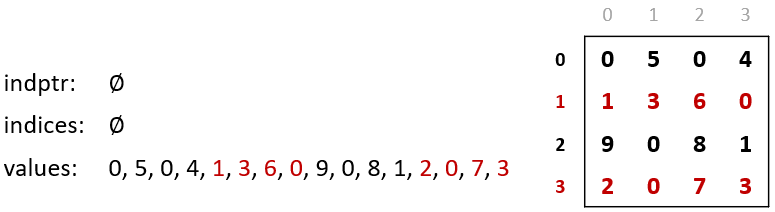
\includegraphics[width=4in]{GrB_DENSE_ROW_FORMAT.png}
    \end{center}
    \vspace{-1em}
    \caption{Data layout for the dense row-major format.}
    \hrule
\end{figure}


\subsection{{\sf GrB\_DENSE\_COL\_FORMAT}}
The {\sf GrB\_DENSE\_COL\_FORMAT} format indicates that a matrix will be imported
or exported using the dense column-major format.  {\sf indptr} and {\sf indices} are unused,
and may be set to NULL, while {\sf values} will point to an array of size number of columns
times number of rows, where element i,j is located at index i + j*nrows.\\

\begin{figure}[h]
    \hrule
    \begin{center}
        ~\\
        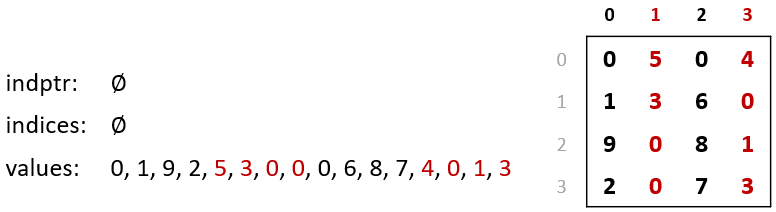
\includegraphics[width=4in]{GrB_DENSE_COLUMN_FORMAT.png}
    \end{center}
    \vspace{-1em}
    \caption{Data layout for the dense column-major format.}
    \label{Fig:formats}
    \hrule
\end{figure}

%--------------------------------------------------------------
%--------------------------------------------------------------

\chapter{Examples}
\label{Chp:Examples}

\pagebreak
\nolinenumbers
\section{Example: level breadth-first search (BFS) in GraphBLAS}
{\scriptsize
\lstinputlisting[language=C,numbers=left]{BFS5M.c}
}
\vfill

\pagebreak
\nolinenumbers
\section{Example: level BFS in GraphBLAS using apply}
{\scriptsize
\lstinputlisting[language=C,numbers=left]{BFS6_apply.c}
}
\vfill

\pagebreak
\nolinenumbers
\section{Example: parent BFS in GraphBLAS}
{\scriptsize
\lstinputlisting[language=C,numbers=left]{BFS7_parents.c}
}
\vfill

\pagebreak
\nolinenumbers
\section{Example: betweenness centrality (BC) in GraphBLAS}
\label{App:BCnobatch}
{\scriptsize
\lstinputlisting[language=C,numbers=left]{BC1M_update.c}
}
\vfill

\pagebreak
\nolinenumbers
\section{Example: batched BC in GraphBLAS}
{\scriptsize
\lstinputlisting[language=C,escapechar=|,numbers=left]{BC1_batch.c}
}
\vfill

\pagebreak
\nolinenumbers
\section{Example: maximal independent set (MIS) in GraphBLAS}
{\scriptsize
\lstinputlisting[language=C,numbers=left]{MIS1.c}
}
\vfill

\pagebreak
\nolinenumbers
\section{Example: counting triangles in GraphBLAS}
{\scriptsize
\lstinputlisting[language=C,numbers=left]{TC1.c}
}
\vfill
\pagebreak

\linenumbers
